\section{Proces a forma}
Ústředním tématem geomorfologie je zkoumání interakcí mezi geomorfologickými procesy a formami reliéfu. Procesy utvářejí georeliéf a naopak georeliéf ovlivňuje geomorfologické procesy. Podívejme se na řeku v horách. Velký sklon říčního koryta (forma) jí dává velkou energii. Řeka tak má poměrně velkou schopnost eroze a transportu materiálu (procesy). V místě zaústění toku do nížin sklon koryta klesá (změna formy) a erozní a transportní schopnost řeky se také snižuje, což způsobuje naopak akumulaci materiálu v předpolí (procesy).

Z forem reliéfu můžeme vyčíst celou řadu informací o procesech, které je utvářely nebo utvářejí. Například z tvaru písečných dun lze zjistit jakého směru vanou převládající větry; charakter říčního koryta nám může napovědět o hydrologickém režimu řeky, kolik a jaké sedimenty unáší a podobně. 

Mnohé formy reliéfu jsou reliktem geomorfologických procesů dob minulých. Díky nim tak můžeme studovat historii a vývoj krajiny. Příkladem mohou být ledovcová údolí, kary a morény ve Vysokých Tatrách -- důkaz přítomnosti ledovců v pleistocénu.

\section{Endogenní a exogenní procesy}
jak již bylo zmíněno, reliéf se vyvíjí působením \emph{geomorfologických procesů}. Tyto procesy dělíme do dvou základních skupin, a to na endogenní a exogenní. \textbf{Endogenní} procesy mají svůj původ v zemském nitru. Jejich hlavní zdroj energie je rozpad radioaktivních prvků v zemském jádře. Projev endogenních procesů je například vulkanismus, zemětřesení, pohyby litosférických desek. \textbf{Exogenní} procesy mají svůj zdroj energie ve Slunci. Uplatňuje se u nich ale i gravitace, zemská rotace a slapové jevy. 

Ve své základní podstatě je georeliéf výsledkem protichůdných působení endogenních a exogenních procesů. Obecně můžeme říct, že endogenní procesy hlavně budují reliéf do výšky (Obr. \ref{fig:zmenyvysky}). Jejich působením vznikají pohoří, sopky a podobně. Zvyšují tak vertikální členitost reliéfu. Vyčleňují se tři  hlavní skupiny endogenních procesů. \emph{Magmatické procesy} zahrnují přesuny roztavených hornin (magmatu) k zemskému povrchu. \emph{Orogeneze} označuje vznik rozsáhlých pásemných pohoří. \emph{Epeirogeneze} je výzdvih velkých území bez zjevného vrásnění či rozlámání hornin. 

Exogenní procesy naopak snižují a zarovnávají zemský reliéf (Obr. \ref{fig:zmenyvysky}). Souhrnně se tomuto procesu říká \emph{denudace}. Denudace zahrnuje jak odnos pevných částic, což je nazýváno jako \emph{eroze}, tak i rozpuštěných látek (\emph{chemická denudace}). Samozřejmě i exogenní procesy mohou lokalizovaně zvyšovat zemský reliéf (např. písečné duny, morény).

\begin{figure}[h]
	\centering
	\includegraphics[width=1\linewidth]{obrazky/uvod/zmeny_vysky}
	\caption{Schéma znázorňující změny v nadmořské výšce způsobené různými exogenními a endogenními procesy. Plusové znaménko znamená nárůst nadmořské výšky a potenciální energie, mínus značí opak. Upraveno podle \textcite{summerfieldGlobalGeomorphologyIntroduction1999}}
	\label{fig:zmenyvysky}
\end{figure}

%\section{Geomorfologický systém}
%\todo[inline]{geomorfologický systém}
%%\begin{myboxgreen}
%%	test boxu
%%\end{myboxgreen}

\section{Měřítko}
\subsection{Prostorové měřítko}
Georeliéf lze studovat v různém \emph{prostorovém měřítku}. V planetárním či kontinentálním měřítku studujeme například celé orogény (např. Andy, Himaláje), rychlost jejich výzdvihu, intenzitu denudačních procesů a vliv klimatu na ně. Při bližším pohledu se dostáváme na regionální (makro) měřítko. Jedná se zpravidla o území s jednotnou geologickou stavbou. Dalším příblížením se zaměřujeme již na dílčí formy reliéfu. Studujeme malá povodí, jednotlivé meandry, písečné duny. Ve větším detailu (mikro měřítko) pak studujeme drobné tvary reliéfu -- štěrkové lavice, zlomový sráz vzniklý jedním zemětřesením, mělké sesuvy. Lze se ale přiblížit ještě více. V největším detailu pak můžeme studovat mikroreliéf např. skalních stěn (příkladem drobných tvarů jsou voštiny). 

Je třeba mít na paměti, že pro každou úroveň prostorového měřítka se uplatňují odlišné metody. Při studiu velkých území využijeme např. dálkový průzkum Země, práci v geografických informačních systémech. Při mikro měřítku se bude výzkum odehrávat ve větší míře na daném místě v terénu. Budeme např. zkoumat odkryvy a odebírat vzorky, které následně zpracujeme v laboratoři za účelem zjištění jejich zrnitosti, obsahu organické hmoty apod.

%\begin{table*}[h]
%	\setlength{\tabcolsep}{0.5pt}
%	\footnotesize
%	\begin{tabularx}{1\textwidth}{@{}llllllllllX@{}}
%		\toprule
%		\multirow{3}{*}{\begin{tabular}[c]{@{}l@{}}Prostorové \\ měřítko\end{tabular}} &
%		\multicolumn{2}{c}{Rozměry} &
%		\multicolumn{4}{c}{Příklady tvarů} &
%		\multicolumn{2}{c}{Hlavní kontrolní faktory} &
%		\multicolumn{2}{c}{\multirow{3}{*}{Časové měřítko}} \\ \cmidrule(lr){2-3} \cmidrule(lr){4-7} \cmidrule(lr){8-9}
%		\multicolumn{1}{c}{} &
%		\multicolumn{1}{c}{\multirow{2}{*}{Lineární}} &
%		\multicolumn{1}{c}{\multirow{2}{*}{Plošné}} &
%		\multicolumn{1}{c}{Endogenní} &
%		\multicolumn{3}{c}{Exogenní} &
%		\multicolumn{1}{c}{\multirow{2}{*}{Endogenní}} &
%		\multicolumn{1}{c}{\multirow{2}{*}{Exogenní}} &
%		\multicolumn{2}{c}{} \\ \cmidrule(lr){5-7} 
%		\multicolumn{1}{c}{} &
%		\multicolumn{1}{c}{} &
%		\multicolumn{1}{c}{} &
%		&
%		\multicolumn{1}{c}{Fluviální} &
%		\multicolumn{1}{c}{Glaciální} &
%		\multicolumn{1}{c}{Eolické} &
%		\multicolumn{1}{c}{} &
%		\multicolumn{1}{c}{} &
%		\multicolumn{2}{c}{} \\ \midrule
%		Mikro &
%		$<0,5$ &
%		$<0,25$ &
%		Malé zlomové svahy &
%		Tůně a peřeje v malém povodí &
%		Malé morénové hřbety &
%		Písečné čeřiny &
%		Jednotlivá zemětřesení nebo sopečné erupce &
%		Mikroklima, meteorologické události &
%		Steady tim &
%		$10^1$ \\ \midrule
%		Meso &
%		$0,5$--$10$ &
%		$0,25$--$10^2$ &
%		Malé sopky &
%		Malá ledovcová údolí &
%		Meandry &
%		Duny &
%		Místní a regionální isostatický výzdvih, lokální vulkanismus a zemětřesení &
%		Lokální klima, krátkodobé změny klimatu &
%		dynamický čas &
%		$10^3$ \\ \midrule
%		Macro &
%		$10$--$10^3$ &
%		$10^2$--$10^6$&
%		Zlomová pohoří  & %Block-faulted terrain
%		Nivy velkých řek &
%		Ledovcové čapky &
%		Písečná moře &
%		Regionální výzdvih a pokles &
%		Regionální klima, dlouhodobé změny klimatu (střídání glaciálů a interglaciálů) &
%		\multirow{2}{*}[-2em]{Cyklický čas} &
%		\multirow{2}{*}{$10^7$} \\ \cmidrule(lr){1-9}
%		Mega &
%		$>10^3$ &
%		$>10^6$ &
%		Hlavní orogény &
%		Hlavní povodí &
%		Kontinentální ledovcové příkrovy &
%		Rozsáhlá písečná moře &
%		Dlouhodobé rozložení výzdvihu, poklesu a pohyby litosférických desek &
%		Hlavní klimatické zóny, dlouhotrvající změny klimatu (doby ledové) &
%		&
%		\\ \bottomrule
%	\end{tabularx}
%	\caption{Hierarchie prostorových a časových měřítek (upraveno podle \textcite{summerfieldGlobalGeomorphologyIntroduction1999})}
%	\label{tab:meritko}
%	
%\end{table*}

\subsection{Časové měřítko}\index{čas}
Vývoj georeliéfu probíhá i v rozličném čase. Některé změny se odehrávají během vteřin, jiné zase trvají milióny let. Zlomový sráz může vzniknout během okamžiku při zemětřesení. Může ale trvat stovky let i tisíce let, než jej eroze zcela zahladí. Rychlost, jakou bude vzniklý stupeň zahlazen závisí na celé řadě faktorů. První faktor ovlivňující životnost tvaru je to, zda prostředí, ve kterém se nachází je charakteristické vysokou mírou eroze a akumulace nebo je to naopak relativně klidné prostředí. V prvním případě může být stupeň zhlazen během několika málo desítek let. V druhém případě bude patrný v reliéfu i po několika staletích. Druhý faktor je odolnost materiálu, ze kterého je tvořen tvar vůči odnosu. Vodní tok v sedimentech bude snáz proměňovat své koryto, než kdyby tekl ve skalním korytě. Třetím faktorem je velikost tvaru. Menší tvary vznikají a zanikají rychleji, než tvary velké. 

\section{Základní teoretická východiska}

\subsection{Zachování hmoty v krajině}
Zemský povrch, georeliéf je dynamickým systémem, skrz který dochází k přesunům hmoty. Hmota nikde nemizí, jen je přemisťována z jednoho místa na druhé. Když se sesune část svahu, dojde k přesunu hmoty z horní části svahu k jeho úpatí. V odlučné oblasti materiál chybí, v akumulační zóně naopak hmoty přibylo. Pro určitou část zemského povrchu za určitou dobu platí: 
\begin{equation}\label{key}
	I-O=\delta ST	
\end{equation}
\begin{eqexpl}
	\item{$I$}vstup hmoty (to co přibylo)
	\item{$O$}výstup hmoty (to co ubylo)
	\item{$\delta ST$}změna zásob hmoty
\end{eqexpl}

Velikost a charakter změny zásob hmoty v určitém území určuje její charakter. Hory, které erodují rychleji než je tektonický výzdvih se snižují. Pokud se do řeky dostává více sedimentů, než je schopna unášet, tak se časem koryto zaplní \parencite{biermanKeyConceptsGeomorphology2014}.

\subsection{Zachování energie}
Energii nelze vyrobit ani zničit, ale pouze přeměnit na jiný druh energie. Potenciální energie daná pozicí v reliéfu se může změnit na kinetickou energii. Když se na svahu uvolní kámen, začne se kutálet dolů. Jeho potenciální energie daná jeho pozicí na svahu se mění v kinetickou energii. Část kinetické energie se mění na teplo z důvodu tření. 

\subsection{Pohyb hmoty}
Pohyb hmoty je od zdrojnice (angl. source) materiálu k místu akumulace (angl. sink). Většinou se jedná o jednosměrný tok z vyšších poloh do nižších. Materiál je unášen řekou z horních částí toku až do sedimentačních pánví (jezero, moře)

\subsection{Rovnováha sil a prahy}
Systém je udržován v dynamické rovnováze celou řadou zpětných vazeb. Narušením systému může dojít k takovému vychýlení, že se již není schopen vrátit zpět na stejnou trajektorii vývoje. Po dílčím období nestability dochází k nastolení nové dynamické rovnováhy a systém se vyvíjí po nové trajektorii.

\begin{figure*}[h]
	\centering
	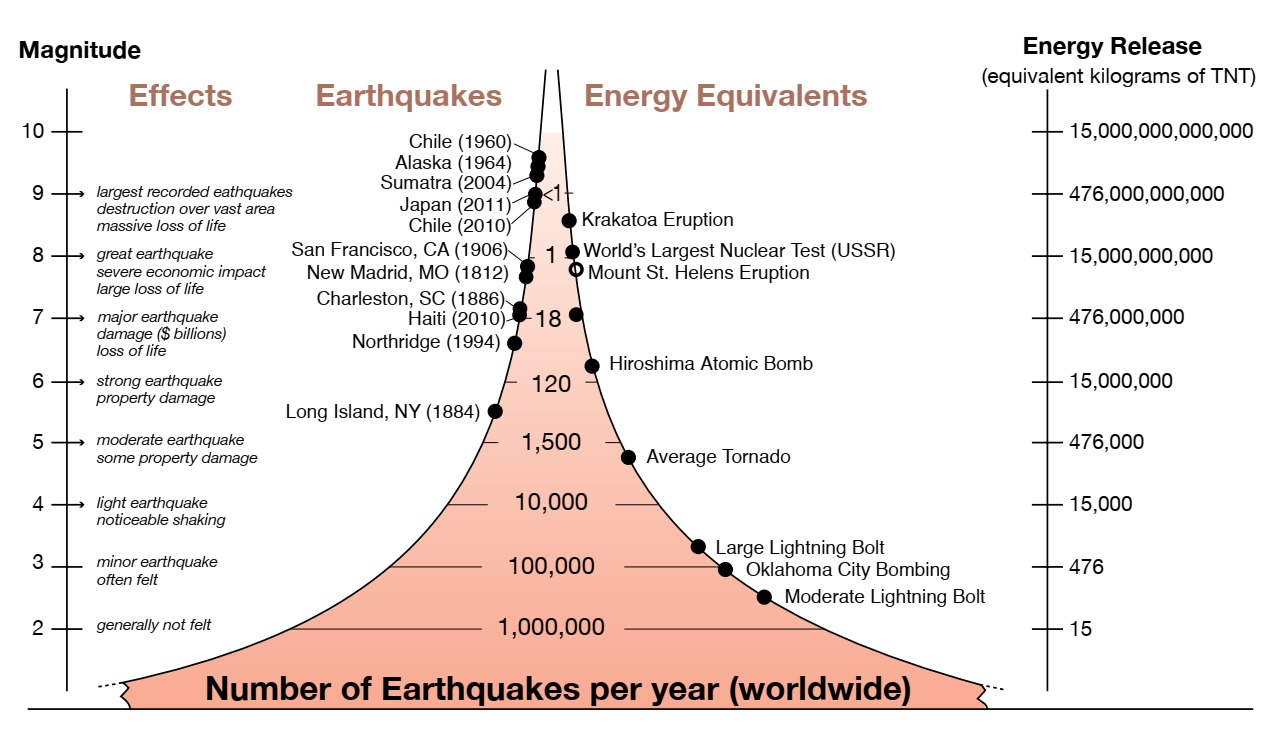
\includegraphics[width=1\linewidth]{obrazky/uvod/frekvence}
	\caption{Četnost zemětřesení (zdroj: IRIS.edu)}
	\label{fig:frekvence}
\end{figure*}

\subsection{Magnitudo a frekvence geomorfologických procesů}
Jevy malého magnituda (rozsahu, intezity...) se dějí často, mají tedy vysokou frekvenci opakování. Příkladem jsou zemětřesení. Slabá zemětřesení (magnitudo 3 a méně) jsou četná (Obr. \ref{fig:frekvence}). Ročně se jich vyskytne $> 1000000$. Silná zemětřesení (magnitudo $>=7$) se vyskytují jen v počtu cca 20 za rok, z k těm nejsilnějším dochází jen jednou za několik let. 
Události malého magnituda nemají zpravidla velký geomorfologický účinek. Naopak jevy velkého magnituda způsobují velké změny v reliéfu, postihují rozsáhlé oblasti apod. Opravdu silných zemětřesení se ročně vyskytne jen pár, ale mají dalekosáhlé důsledky jak pro společnost, tak pro georeliéf.


%\newpage
%\onecolumn
%\begin{boxotazky}{Kontrolní a klíčové otázky, na které bychom měli znát odpověď}
%	\begin{itemize}
%		\item Vysvětlete pojmy proces a forma. Jak spolu souvisí?
%		\item 
%		
%	\end{itemize}
%\end{boxotazky}
%
%\begin{boxslovnik}{Další klíčové pojmy k zapamatování}
%	proces & forma \\
%	endogenní & exogenní \\
%	denudace & eroze
%\end{boxslovnik}
%\twocolumn